\documentclass[tikz,border=10pt]{standalone}
\usepackage{tikz}
\usetikzlibrary{shapes.geometric, arrows.meta, positioning}

\tikzset{
    register/.style={
        rectangle, draw=black, thick,
        minimum width=1.1cm, minimum height=0.8cm,
        fill=white, font=\small\ttfamily
    },
    mux/.style={
        trapezium, trapezium left angle=70, trapezium right angle=110,
        draw=black, thick,
        minimum width=0.9cm, minimum height=0.7cm,
        fill=white, font=\small
    },
    memory/.style={
        rectangle, draw=black, very thick,
        minimum width=1.3cm, minimum height=0.85cm,
        fill=white, font=\small
    },
    wire/.style={draw=black, thick, -Stealth},
    bus/.style={draw=black, line width=1.5pt, -Stealth},
    buswidth/.style={font=\tiny, fill=white, inner sep=1pt},
    logic/.style={
        rectangle, draw=black, thick, rounded corners=3pt,
        minimum width=1.1cm, minimum height=0.75cm,
        fill=gray!10, font=\small
    },
    sbox/.style={
        rectangle, draw=black, thick,
        minimum width=0.65cm, minimum height=0.65cm,
        fill=gray!20, font=\small
    }
}

\begin{document}
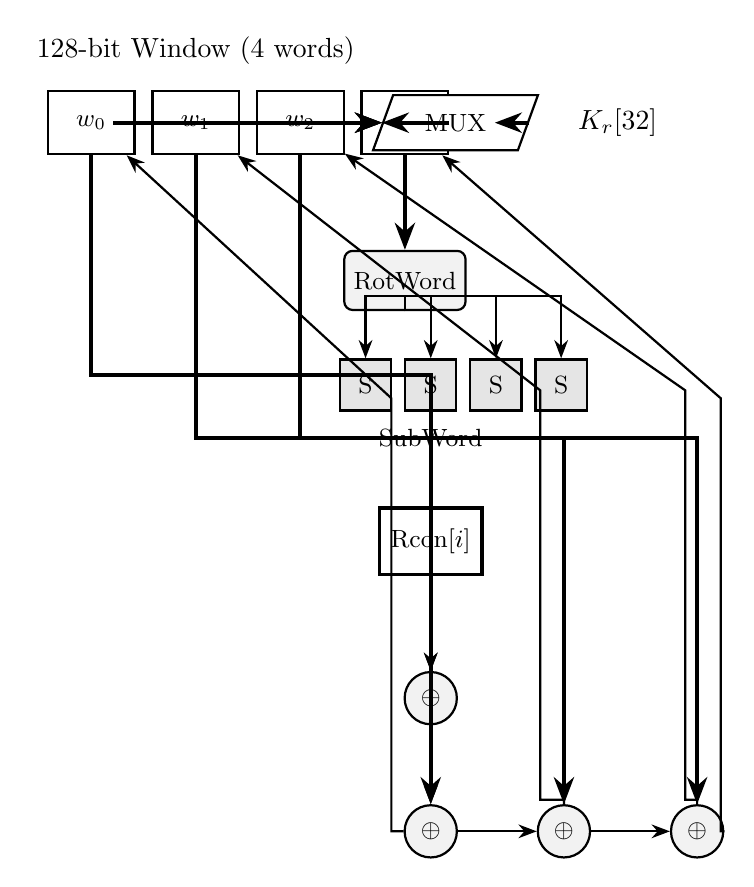
\begin{tikzpicture}[node distance=0.9cm and 1.2cm]

% Key word registers (top row)
\node[register] (w0) at (0,0) {$w_0$};
\node[register, right=0.2cm of w0] (w1) {$w_1$};
\node[register, right=0.2cm of w1] (w2) {$w_2$};
\node[register, right=0.2cm of w2] (w3) {$w_3$};

\node[font=\normalsize, above=0.2cm of w1.north] {128-bit Window (4 words)};

% RotWord operation
\node[logic, below=1.2cm of w3] (rot) {RotWord};

% SubWord S-boxes
\node[sbox, below=0.6cm of rot, xshift=-0.5cm] (s0) {S};
\node[sbox, right=0.15cm of s0] (s1) {S};
\node[sbox, right=0.15cm of s1] (s2) {S};
\node[sbox, right=0.15cm of s2] (s3) {S};
\node[font=\small, below=0.1cm of s1.south] {SubWord};

% Rcon
\node[memory, below=1.2cm of s1] (rcon) {Rcon[$i$]};

% XOR chain
\node[logic, circle, minimum size=0.6cm, below=1.2cm of rcon] (x1) {$\oplus$};
\node[logic, circle, minimum size=0.6cm, below=1cm of x1] (x2) {$\oplus$};
\node[logic, circle, minimum size=0.6cm, right=1cm of x2] (x3) {$\oplus$};
\node[logic, circle, minimum size=0.6cm, right=1cm of x3] (x4) {$\oplus$};

% Connections - RotWord to SubWord
\draw[bus] (w3) -- (rot);
\draw[wire] (rot) -- ++(0,-0.2) -| (s0);
\draw[wire] (rot) -- ++(0,-0.2) -| (s1);
\draw[wire] (rot) -- ++(0,-0.2) -| (s2);
\draw[wire] (rot) -- ++(0,-0.2) -| (s3);

% XOR chain connections
\draw[wire] (s1) -- ++(0,-0.4) -| (x1);
\draw[wire] (rcon) -- (x1);
\draw[bus] (w0) -- ++(0,-3.2) -| (x2);
\draw[wire] (x1) -- (x2);
\draw[wire] (x2) -- (x3);
\draw[bus] (w1) -- ++(0,-4) -| (x3);
\draw[bus] (w2) -- ++(0,-4) -| (x4);
\draw[wire] (x3) -- (x4);

% Feedback paths
\draw[wire] (x2) -- ++(-0.5,0) -- ++(0,5.5) -- (w0);
\draw[wire] (x3) -- ++(0,0.4) -- ++(-0.3,0) -- ++(0,5.2) -- (w1);
\draw[wire] (x4) -- ++(0,0.4) -- ++(-0.15,0) -- ++(0,5.2) -- (w2);
\draw[wire] (x4) -- ++(0.3,0) -- ++(0,5.5) -- (w3);

% Output MUX
\node[mux, right=1.8cm of w1] (outmux) {MUX};
\draw[bus] (w0) -- ++(0.3,0) |- (outmux);
\draw[bus] (w1) -- ++(0.35,0) |- (outmux);
\draw[bus] (w2) -- ++(0.4,0) |- (outmux);
\draw[bus] (w3) -- ++(0.45,0) |- (outmux);
\node[right=0.5cm of outmux, font=\normalsize] {$K_r$[32]};
\draw[bus] (outmux) -- ++(0.5,0);

\end{tikzpicture}
\end{document}
